\subsubsection{Diferencia de frecuencias absolutas}
Como bien apuntan \cite{monroe2008fightin}, esta comparación no resulta tan rica
a la hora de contrastar lemas empleados por los distintos conjuntos de
votantes puesto que se ve fuertemente influenciada por la cantidad y longitud
de los discursos emitidos por cada grupo.
\par
En nuestro caso, se observa que la mayor\'ia de los lemas son característicos
del grupo de los votantes positivos, pero esto es una consecuencia del hecho
de que es el conjunto de estos votantes precisamente el que mayor cantidad de
discursos emitió, así como también, de mayor longitud, como muestra la distribución
de la figura \ref{fig-distrib-unique-tokens}. Asimismo, vemos en la figura
\ref{fig-statistics-freq-abs} que las palabras identificadas como características
de cada grupo (las azules, de los votantes a favor y las rojas, de los votantes
en contra) no resultan significativas, puesto que la mayoría de ellas constituyen
palabras con escaso o nulo significado semántico (son verbos como `tener' o
determinantes, como `el' o `la').

\begin{figure}[h!]
    \centering
    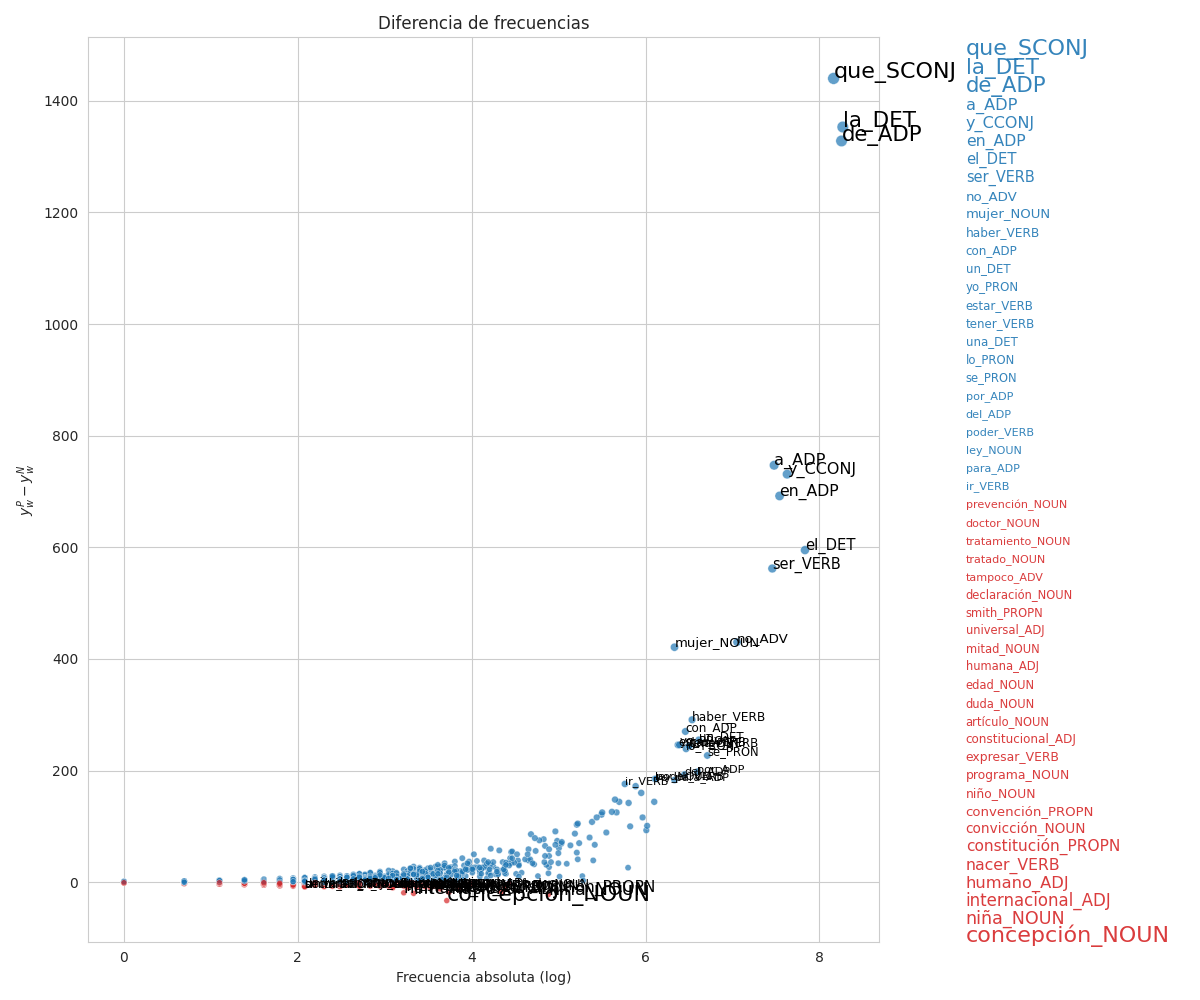
\includegraphics[scale=0.55]{../visualizations/stats/frecuencias.png}
    \caption{Comparación de palabras características de los votos afirmativos y
    negativos tomando como medida la diferencia de frecuencias absolutas descripta
    en la sección \ref{subsubsect-freq-abs}. El eje de abscisas indica el logaritmo
    de la frecuencia absoluta de cada palabra en el conjunto de total de discursos
    y el eje de ordenadas, la comparación en cuestión. En la columna de la
    derecha se observan las 25 palabras más representativas de cada grupo de
    votantes escaladas según su relevancia.}
    \label{fig-statistics-freq-abs}
\end{figure}

\subsubsection{Diferencia de proporciones}

\subsubsection{Ratio de \textit{Odds}}

\subsubsection{Ratio \textit{Log-odds}}

\subsubsection{\textit{TF-IDF}}

\subsubsection{\textit{Word Scores}}


% gráficos que debería mostrar en la des de
% los datos porque son funcionales a esta sección
% --- cantidad de votantes de cada intención de voto
% --- cantitdad de discursos emitidos por cada grupo
% --- longitud de los discursos emitidos